\section{Evaluating Impact of Stream Size on $\Theta$ Sketch}
\label{sec:eval}
We continue with the $\Theta$ sketch experimentation to demonstrate the impact of the stream size on accuracy and performance. 
%We compare the concurrent theta sketch to a sequential Theta sketch wrapped with a reader-writer lock. 
In these experiments the hardware is a 12-core Intel Xeon E5-2620 machine.
Experiment set-up is described in Section~\ref{ssec:setup}. We then discuss accuracy and performance results. Finally, Section~\ref{ssec:tradeoffs} presents tradeoffs between accuracy and performance, which demonstrate the benefits of our stream size-adaptive algorithm.

\subsection{Setup}
\label{ssec:setup}
\paragraph{Implementation}
Concurrent $\Theta$ sketch is implemented in Java as part of the Apache DataSketches (incubating) project, and is generally available since V0.13.0. 
%We compare it to the sequential Theta sketch wrapped with a reader-writer lock.
The sequential implementation and the sketch at the core of the global sketch in the concurrent implementation are the same (HeapQuickSelectSketch, which is the default sketch family).

Global sketch defines \emph{exact limit} -- the limit between exact mode (eager propagation) and estimate mode (lazy propagation). The limit is a function of a configurable error parameter $e$; the function used in the library is $2/e^2$. 
%
Local sketch defines $b$ to be a function of $k$, $e$ and the maximum number of local threads $N$. $b$ has positive correlation with $e$ and inverse correlation with $N$.

Eager propagation, as described in the pseudo-code, requires context switch which incurs high overhead. In the implementation, either the local thread itself eagerly executes every update to the global sketch (buffer size is 1) or lazily delegates updates to a background propagation thread (buffer size is $b$). The decision is based on the global sketch mode (exact or estimate), which is cached in the local sketch as part of the piggyback process that also updates local theta. 
As long as the global sketch is in exact mode the propagation critical section is protected by a shared boolean flag indicating whether (eager) propagation is in progress. When the global sketch switches to estimate mode it is guaranteed that no eager propagation gets through; instead local threads attempting to update the global sketch via eager propagation get an indication to pass the buffer via lazy propagation.
This implementation ensures (a) local threads avoid costly context switch when the sketch is small, (b) lazy propagation by a background thread is done without synchronization.

Unless otherwise stated sketches are configured with $k = 4096$, and $e=0.04$; Thus the exact limit is $2/e^2=1250$, and $b$ is set (by the implementation) to a value between 1 and 5 to accommodate the error bound.


\paragraph{Workload}
We focus on two simple workloads: (1) write-only  - updating a sketch with a stream of unique ids; (2) mixed read-write workload - updating
a sketch with background readers querying the number of unique ids in the stream. Background reads refer to threads that occasionally
(with 1 ms pauses) query the sketch. This simulates real world scenario where updates are constantly streaming from a feed or multiple
feeds, while queries arrive at lower rate.

In both write-only and read-write workloads we measure only the throughput. We vary the number of threads used to feed
the sketch between 1 to 12. In all read-write benchmarks we exercise 10 background reader threads.
\remove{
We refrain from measuring latency of read operations first, since it is challenging (capturing the duration of a few nanoseconds operation).
Second, while it is clear that reading the state of a Theta sketch without a lock is more efficient than doing so after acquiring a lock,
the effect on the entire end-to-end read operation which may include network latencies is negligible. Therefore, we focus on the effect of locks on ingestion throughput.
}
\paragraph{Framework}
To run the experiments we employ a multi-thread extension of the characterization framework. This is the Apache DataSketch evaluation benchmark suite, which measures both the speed and accuracy of the sketch. 

For measuring write throughput the sketch is fed with a continuous data stream. The size of the stream varies from 1 to 8M uniques. For each size $x$ we measure the time $t$ it takes to feed the sketch $x$ unique values, and present it in term of throughput ($x/t$). To avoid measurements noise, each point on the graph represents an average of many trials. The number of trials is very high ($2^{18}$) for points at the low end of the graph. It gradually decreases as the size of the sketch increases. At the high end (at 8M uniques per trial) the number of trials is 16. 

Accuracy of concurrent $\Theta$ sketch is measured only in a single-thread environment. As in the performance evaluations the $x$-axis represents the number of uniques fed into a sketch by a single writing thread. For each size $x$ one trial logs the estimation result after feeding x unique values to the sketch. In addition, it logs the Relative Error (RE) of the estimate, where RE = MeasuredValue/TrueValue -1. This trial is repeated multiple times (specifically 4K times), logging all estimation and RE results. The $y$-axis are the lines of the mean and some constant quantiles of the distributions of error measured at each $x$-axis point on the graph, including the median. 
This type of graph is called ``pitchfork''. 
\remove{
Example of accuracy plots for the sequential $\Theta$ sketch can be found in~\cite{accuracy-plots}.
}

\subsection{Results}
\label{ssec:res}

\paragraph{Accuracy Results}
The accuracy result of a concurrent $\Theta$ sketch that does not employ eager propagation are presented in Figure~\ref{fig:accuracy}. There are two interesting phenomena to observe. First, it is interesting to see empirical evaluation reflecting the theoretical analysis presented in Section~\ref{ssec:theta-analysis}, and thus the ``pitchfork'' is distorted toward lower estimation. More specifically, mean relative error is smaller than $0$ and values of relative error in all measured quantiles tend to be smaller than the relative error of a sequential implementation (estimating less than a sequential implementation). Thereby increasing or decreasing the absolute error depending on whether the error is negative or positive.

Second, for small streams, when the number of unique items is lower than $2k$, $\theta=1$ and the estimation is simply the number of items propagated to the global sketch. If eager propagation is not applied, the number of items in the global sketch depends on the delay in propagation. The smaller the sketch is the more significant the delay is, and the mean error reaches as high as 94\% (we capped the error in the figure at 10\%). As the size of the sketch becomes closer to $2k$ the delay in propagation (of last 16 updates) is less significant, and the mean error decreases.
Obviously, most analytic systems today cannot tolerate such high error. For this the algorithm applies eager propagation until the global sketch reaches the desired exact limit. 
Figure~\ref{fig:accuracy-adaptive} depicts the accuracy results when applying eager propagation. Indeed, the error at small streams (smaller than 8k unique items) is less than 4\%.
%This guided us in introducing the adaptive flavour of the algorithm (discussed in Section~\ref{sec:small-streams}) whose performance results are presented in the next section.

\begin{figure*}[tb]
\setlength{\abovecaptionskip}{0pt}
\setlength{\belowcaptionskip}{0pt}
\setlength\textfloatsep{0pt}
\centering
\begin{subfigure}{\columnwidth}\centering
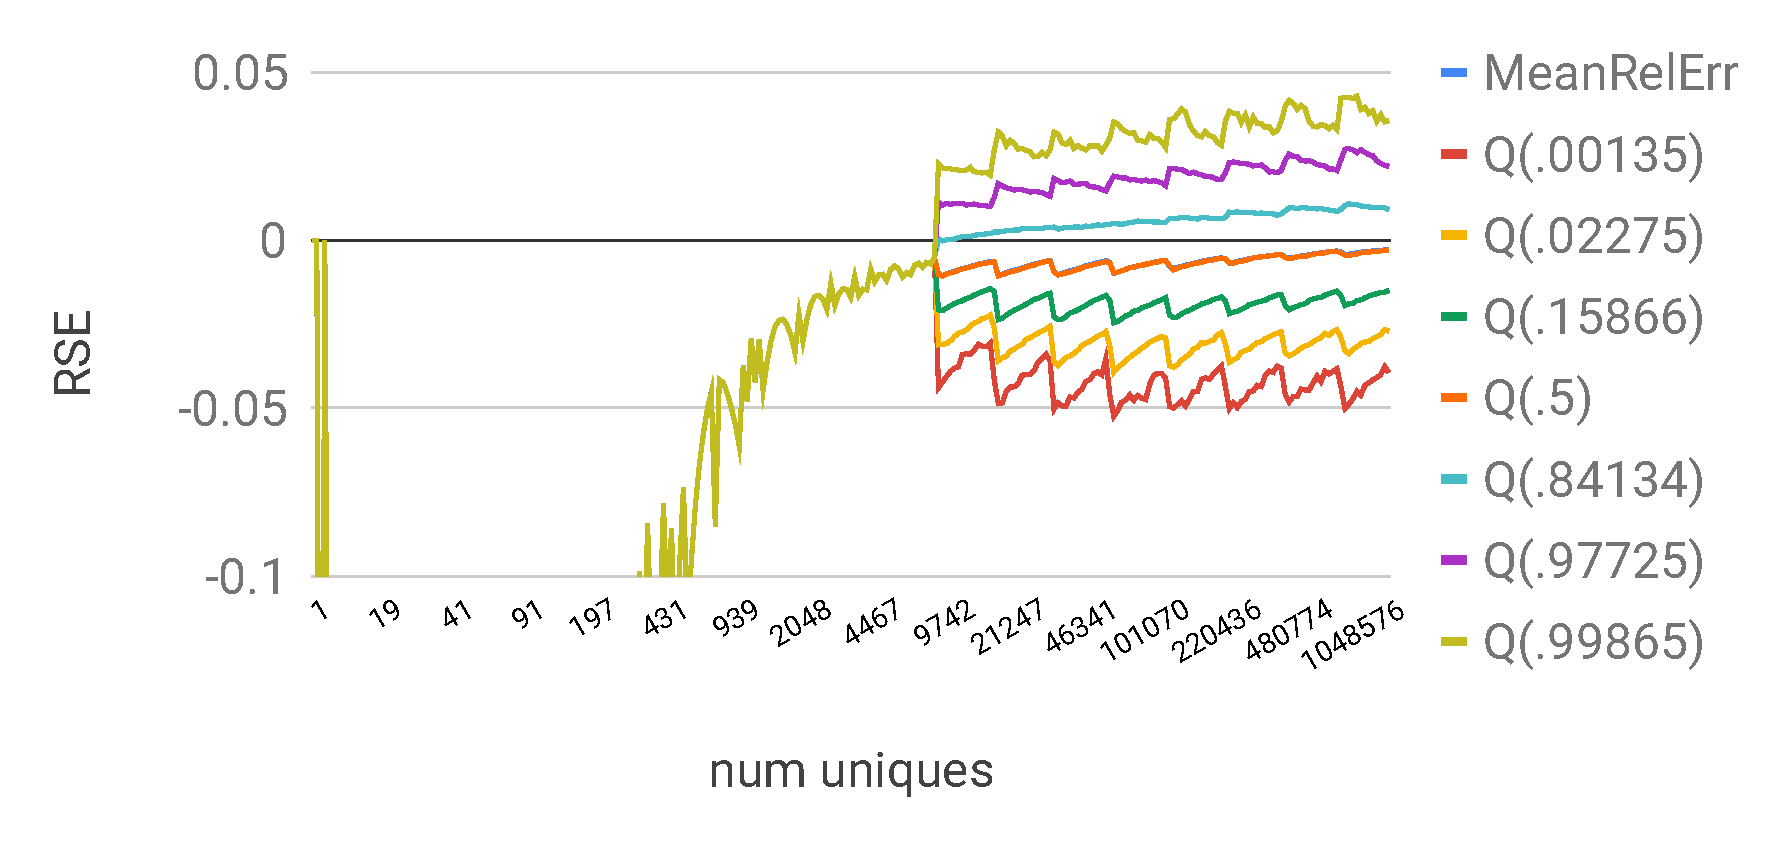
\includegraphics[width=\textwidth]{images/theta-accuracy.pdf}
\caption{No eager propagation ($e=1.0$)}
\label{fig:accuracy}
\end{subfigure}
\begin{subfigure}{\columnwidth}\centering
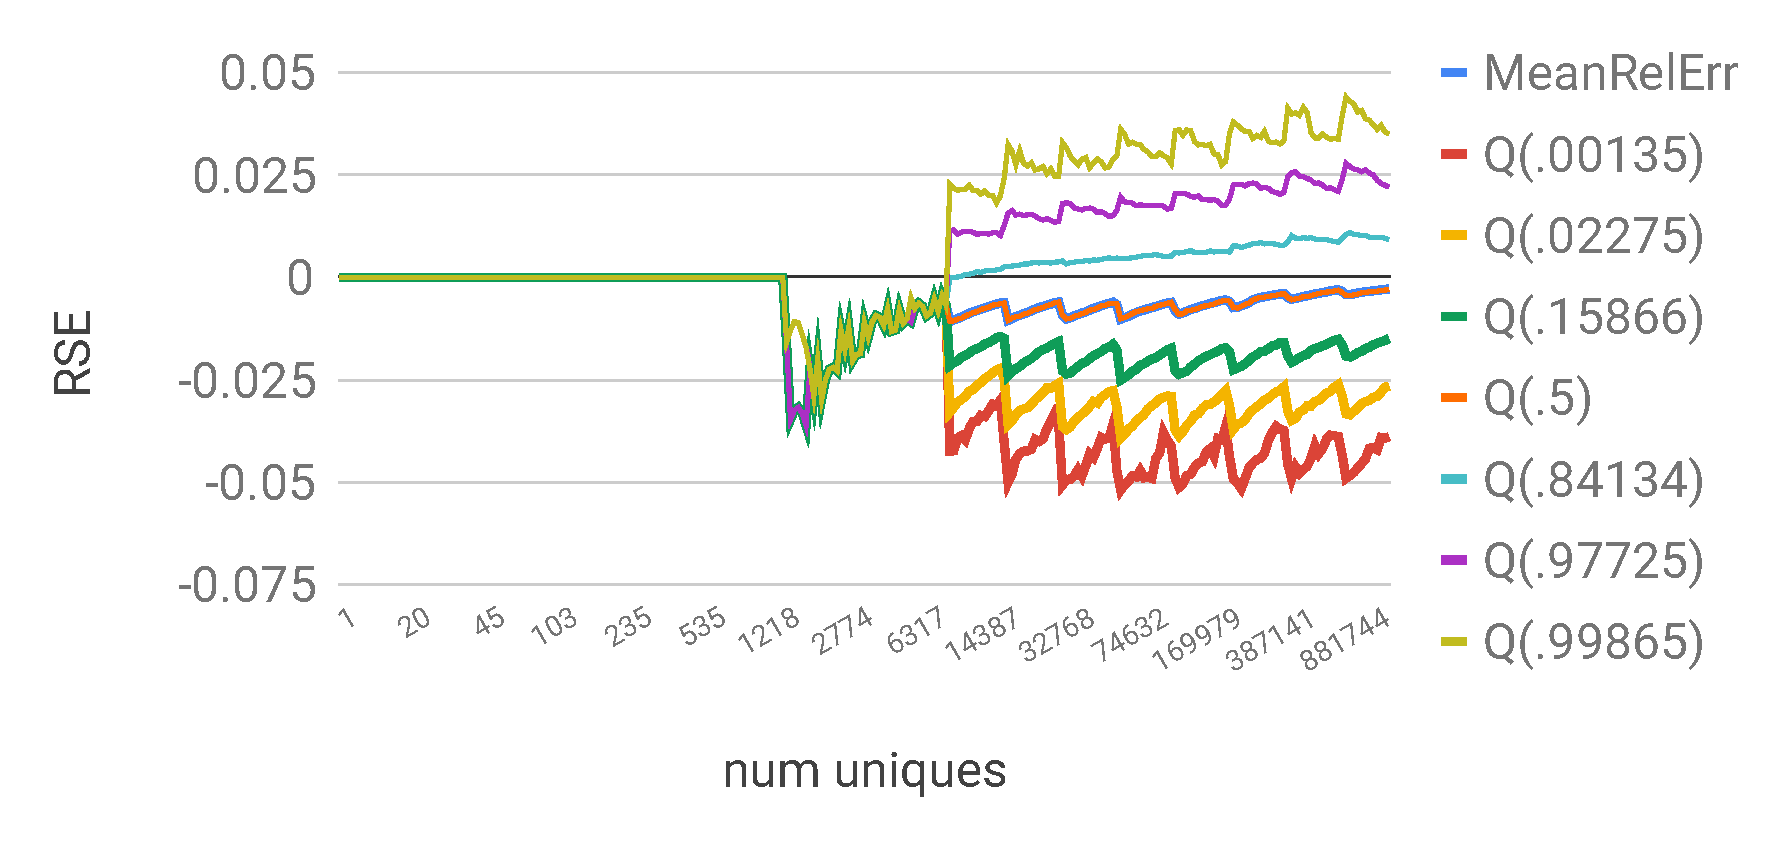
\includegraphics[width=\textwidth]{images/theta-accuracy-adaptive.pdf}
\caption{With eager propagation, limit defined by $e=0.04$}
\label{fig:accuracy-adaptive}
\end{subfigure}
  \caption{Concurrent Theta Measured Quantiles vs RSE, $k = 4096$.}
  \label{fig:accuracy-res}
\end{figure*}

\paragraph{Write-only Throughput}
Figure~\ref{fig:throughput:native} presents throughput measurements of write-only workload. The results are shown in loglog scale.
%It compares concurrent theta implementation vs. lock-based theta implementation. 
Figure~\ref{fig:throughput:large} zooms-in on the throughput of large sketches.

When considering large sketches, the concurrent implementation scales with the number of threads; peaking at almost 300M ops/sec with 12 threads. The performance of lock-based implementation, on the other hand, degrades as the contention on the lock increases with the number of threads. Its peak performance is at 25M ops/sec with a single thread. Namely, the concurrent $\Theta$ sketch outperforms lock-based implementation by 12x, and when comparing the performance of 12 threads, concurrent implementation outperforms lock-based implementation by more than 45x. 

For small streams, wrapping a single thread with a lock is the most efficient method. When the stream contains more than 200K unique values, using concurrent sketch with 4 or more local threads is more efficient. The crossing point of a single local buffer over lock-based implementation is arround 700K uniques.
 
\begin{figure*}[tb]
\setlength{\abovecaptionskip}{0pt}
\setlength{\belowcaptionskip}{0pt}
\setlength\textfloatsep{0pt}
\centering
\begin{subfigure}{1.3\columnwidth}\centering
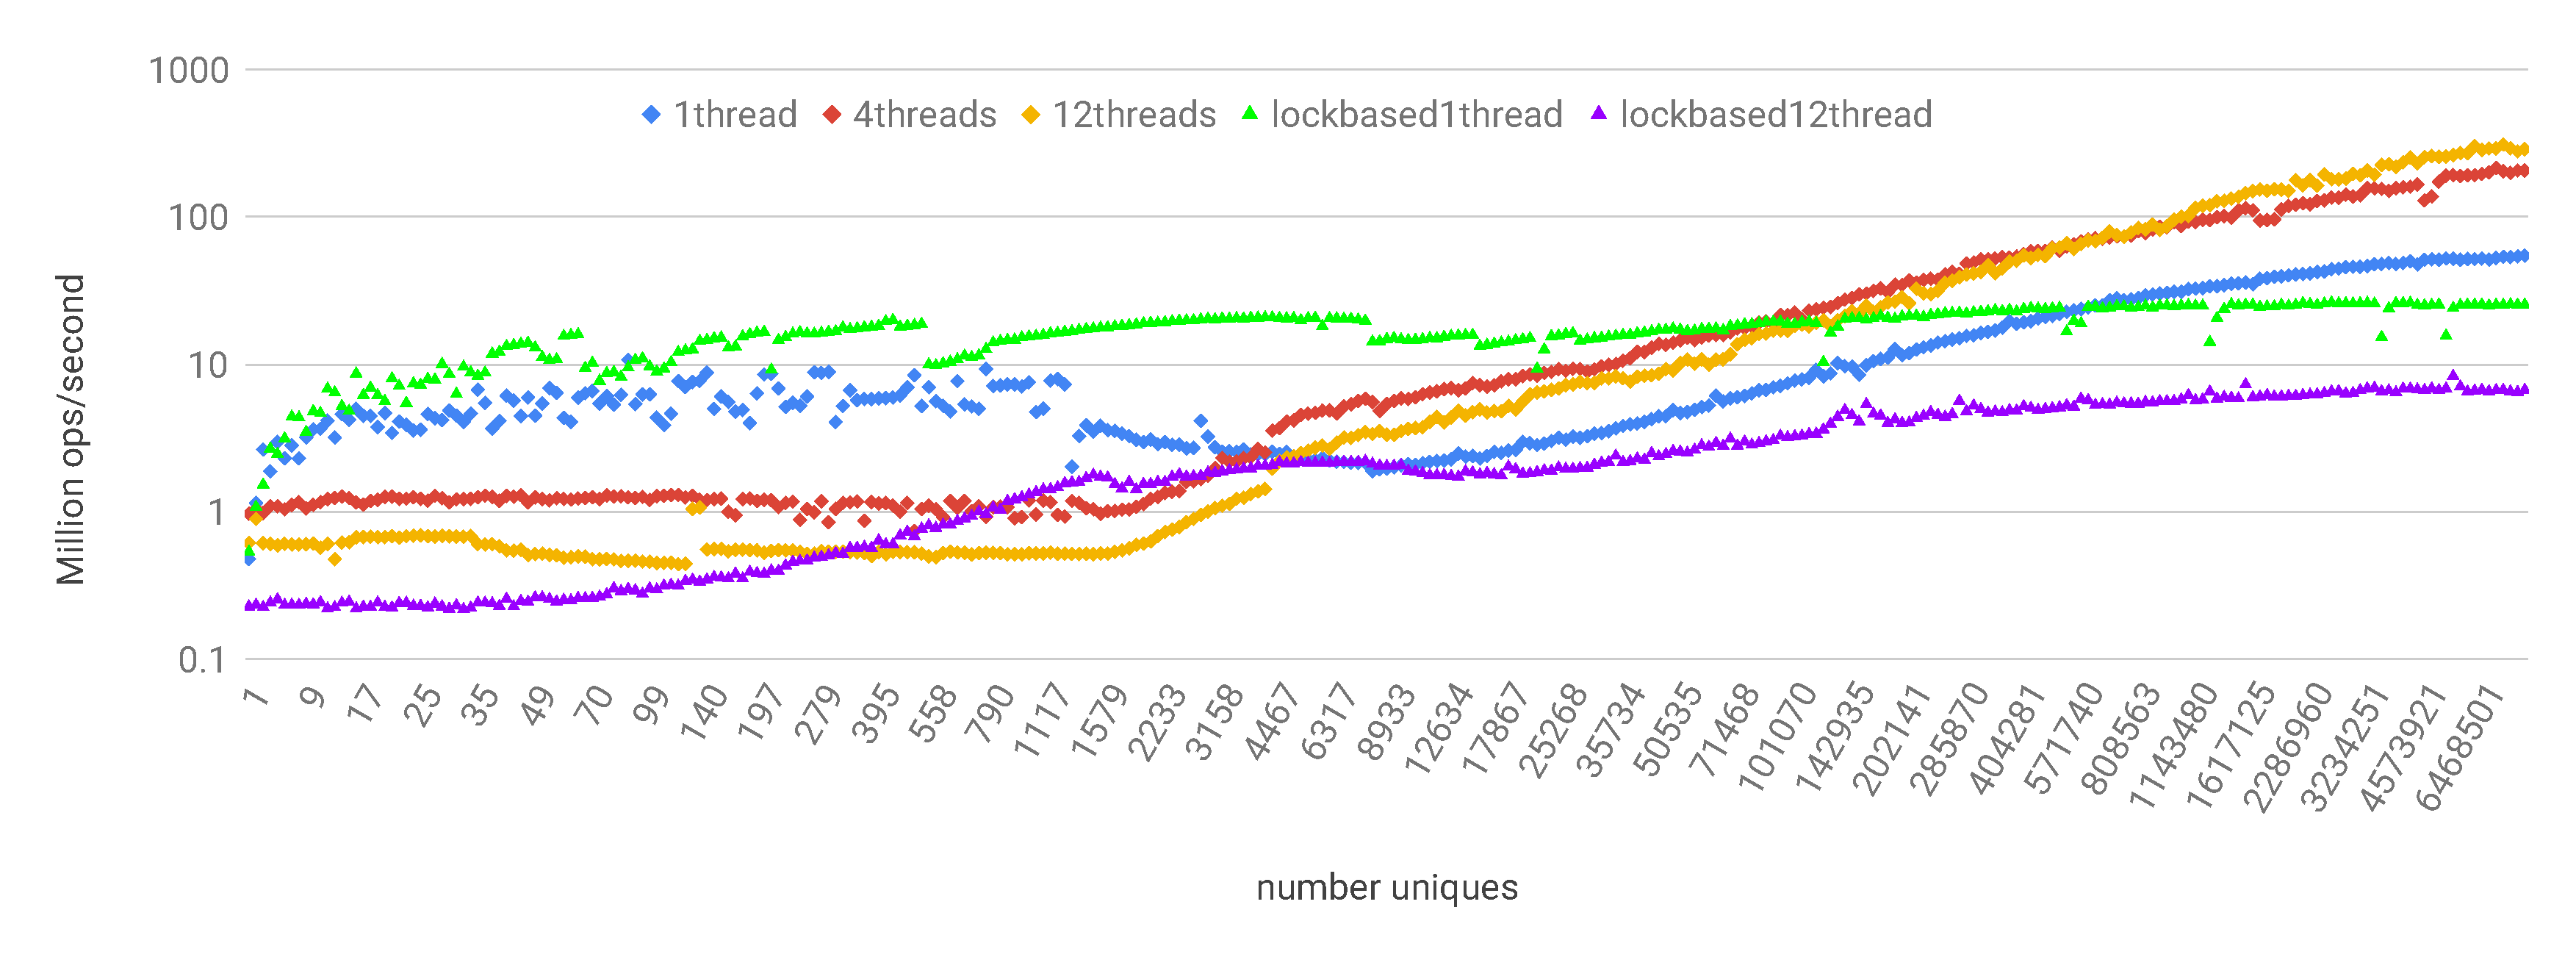
\includegraphics[width=\textwidth]{images/theta-write-only.pdf}
\caption{Throughput, loglog scale}
\label{fig:throughput:native}
\end{subfigure}
\begin{subfigure}{0.7\columnwidth}\centering
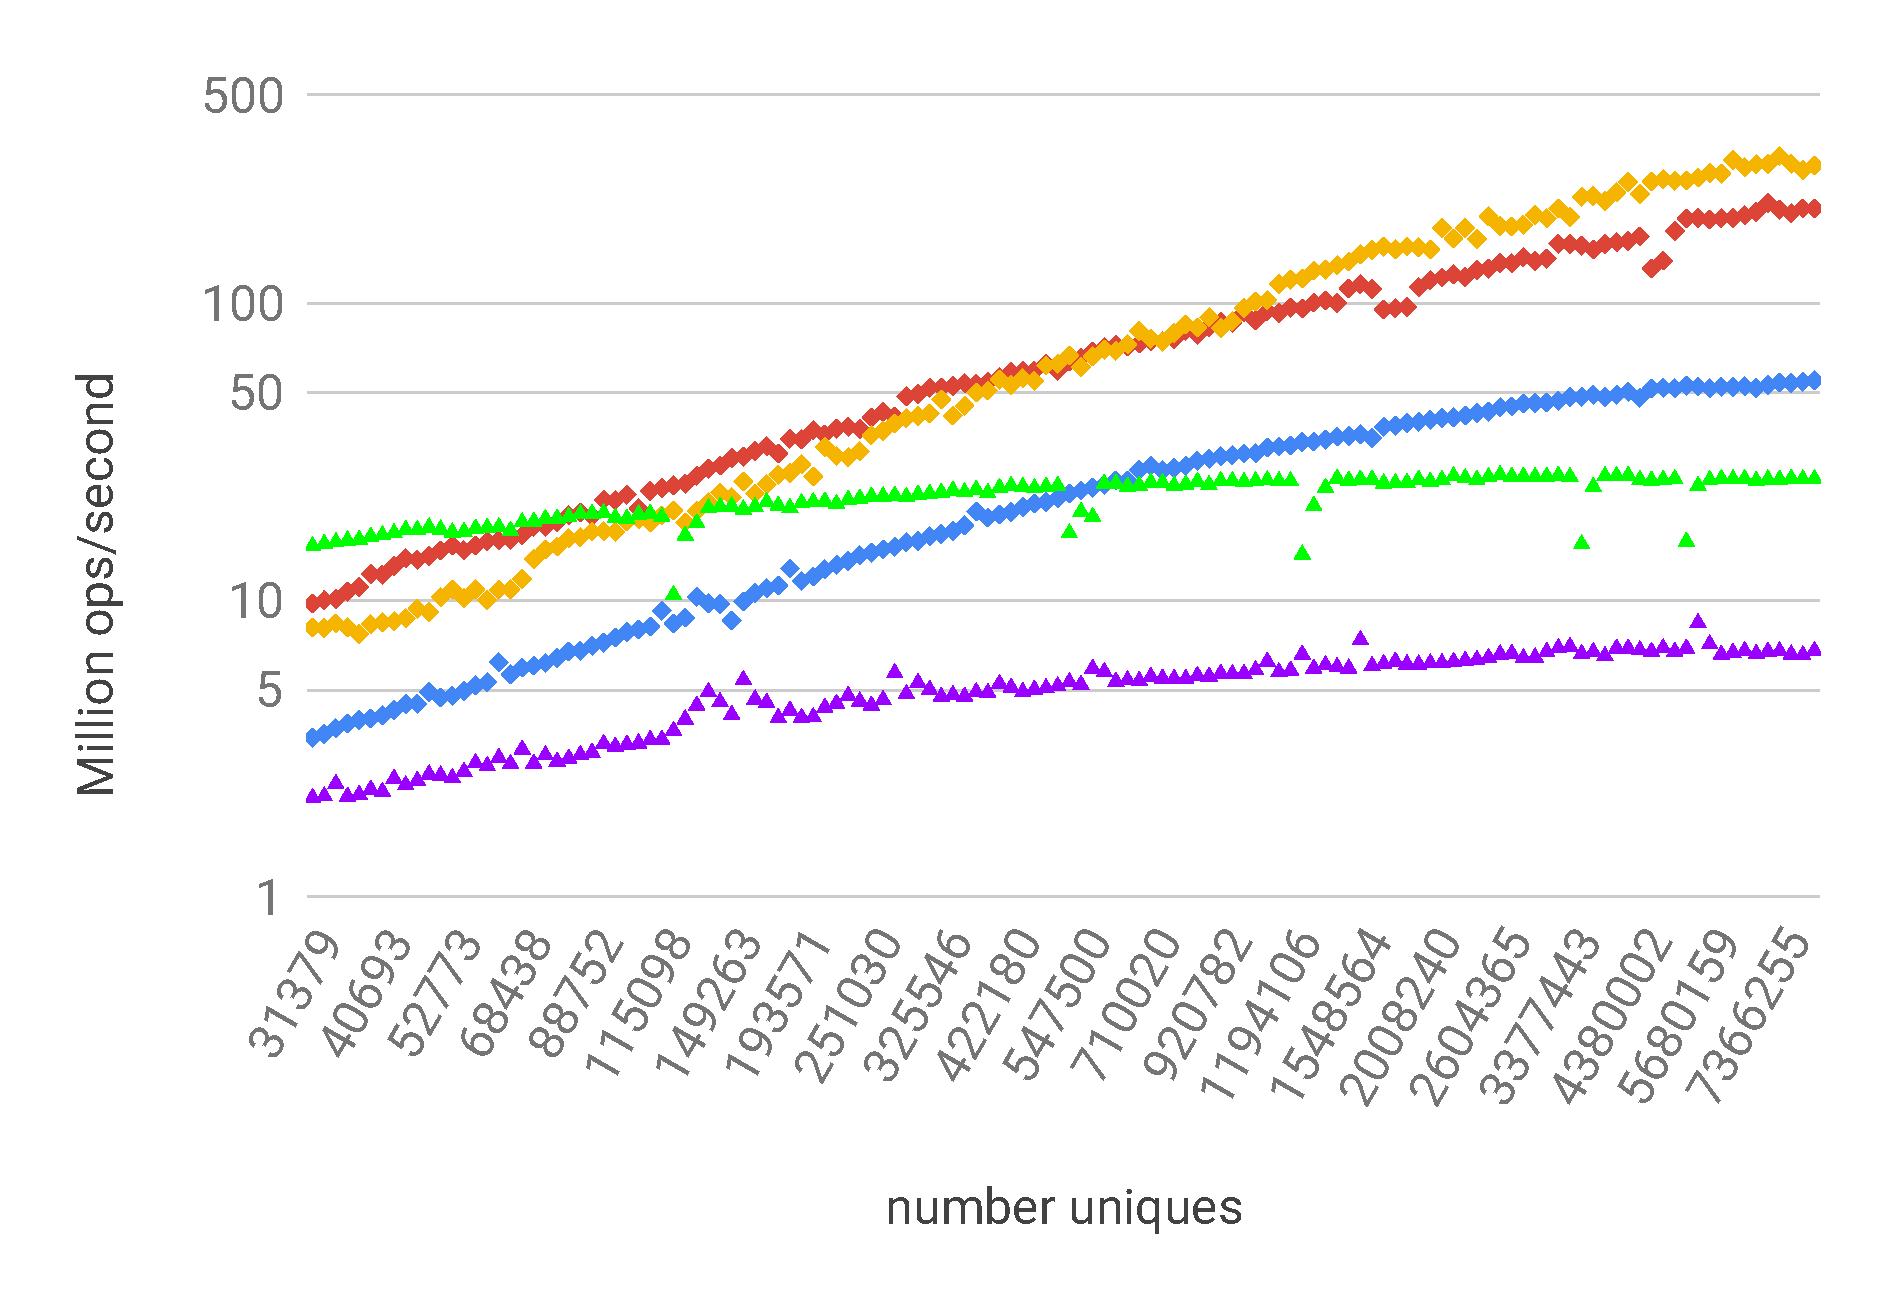
\includegraphics[width=\textwidth]{images/theta-write-only-zoomin.pdf}
\caption{Zooming-in on large sketches}
\label{fig:throughput:large}
\end{subfigure}
  \caption{Write-only workload, $k = 4096$, $e=0.04$.}
  \label{fig:throughput}
\end{figure*}

\paragraph{Mixed Workload}
Figure~\ref{fig:mixed-throughput} presents throughput measurements of mixed read-write workload. We compare runs with a single updating thread and 2 updating threads (and 10 background reader threads).
Here we see similar trends as in the write-only workload. However, the effect of  background readers is more pronounced in lock-based implementation than in concurrent $\Theta$ sketch. The peak throughput of a single writer-thread in the concurrent implementation is 55M ops/sec with and without background readers. The peak throughput of a single writer thread in the lock-based implementation degrades from 25M to 23M ops/sec; almost $10$\% slowdown in performance. And recall that this is when readers are not very frequent.

\begin{figure}[tb]
\setlength{\abovecaptionskip}{0pt}
\setlength{\belowcaptionskip}{0pt}
\setlength\textfloatsep{0pt}
	\centering
	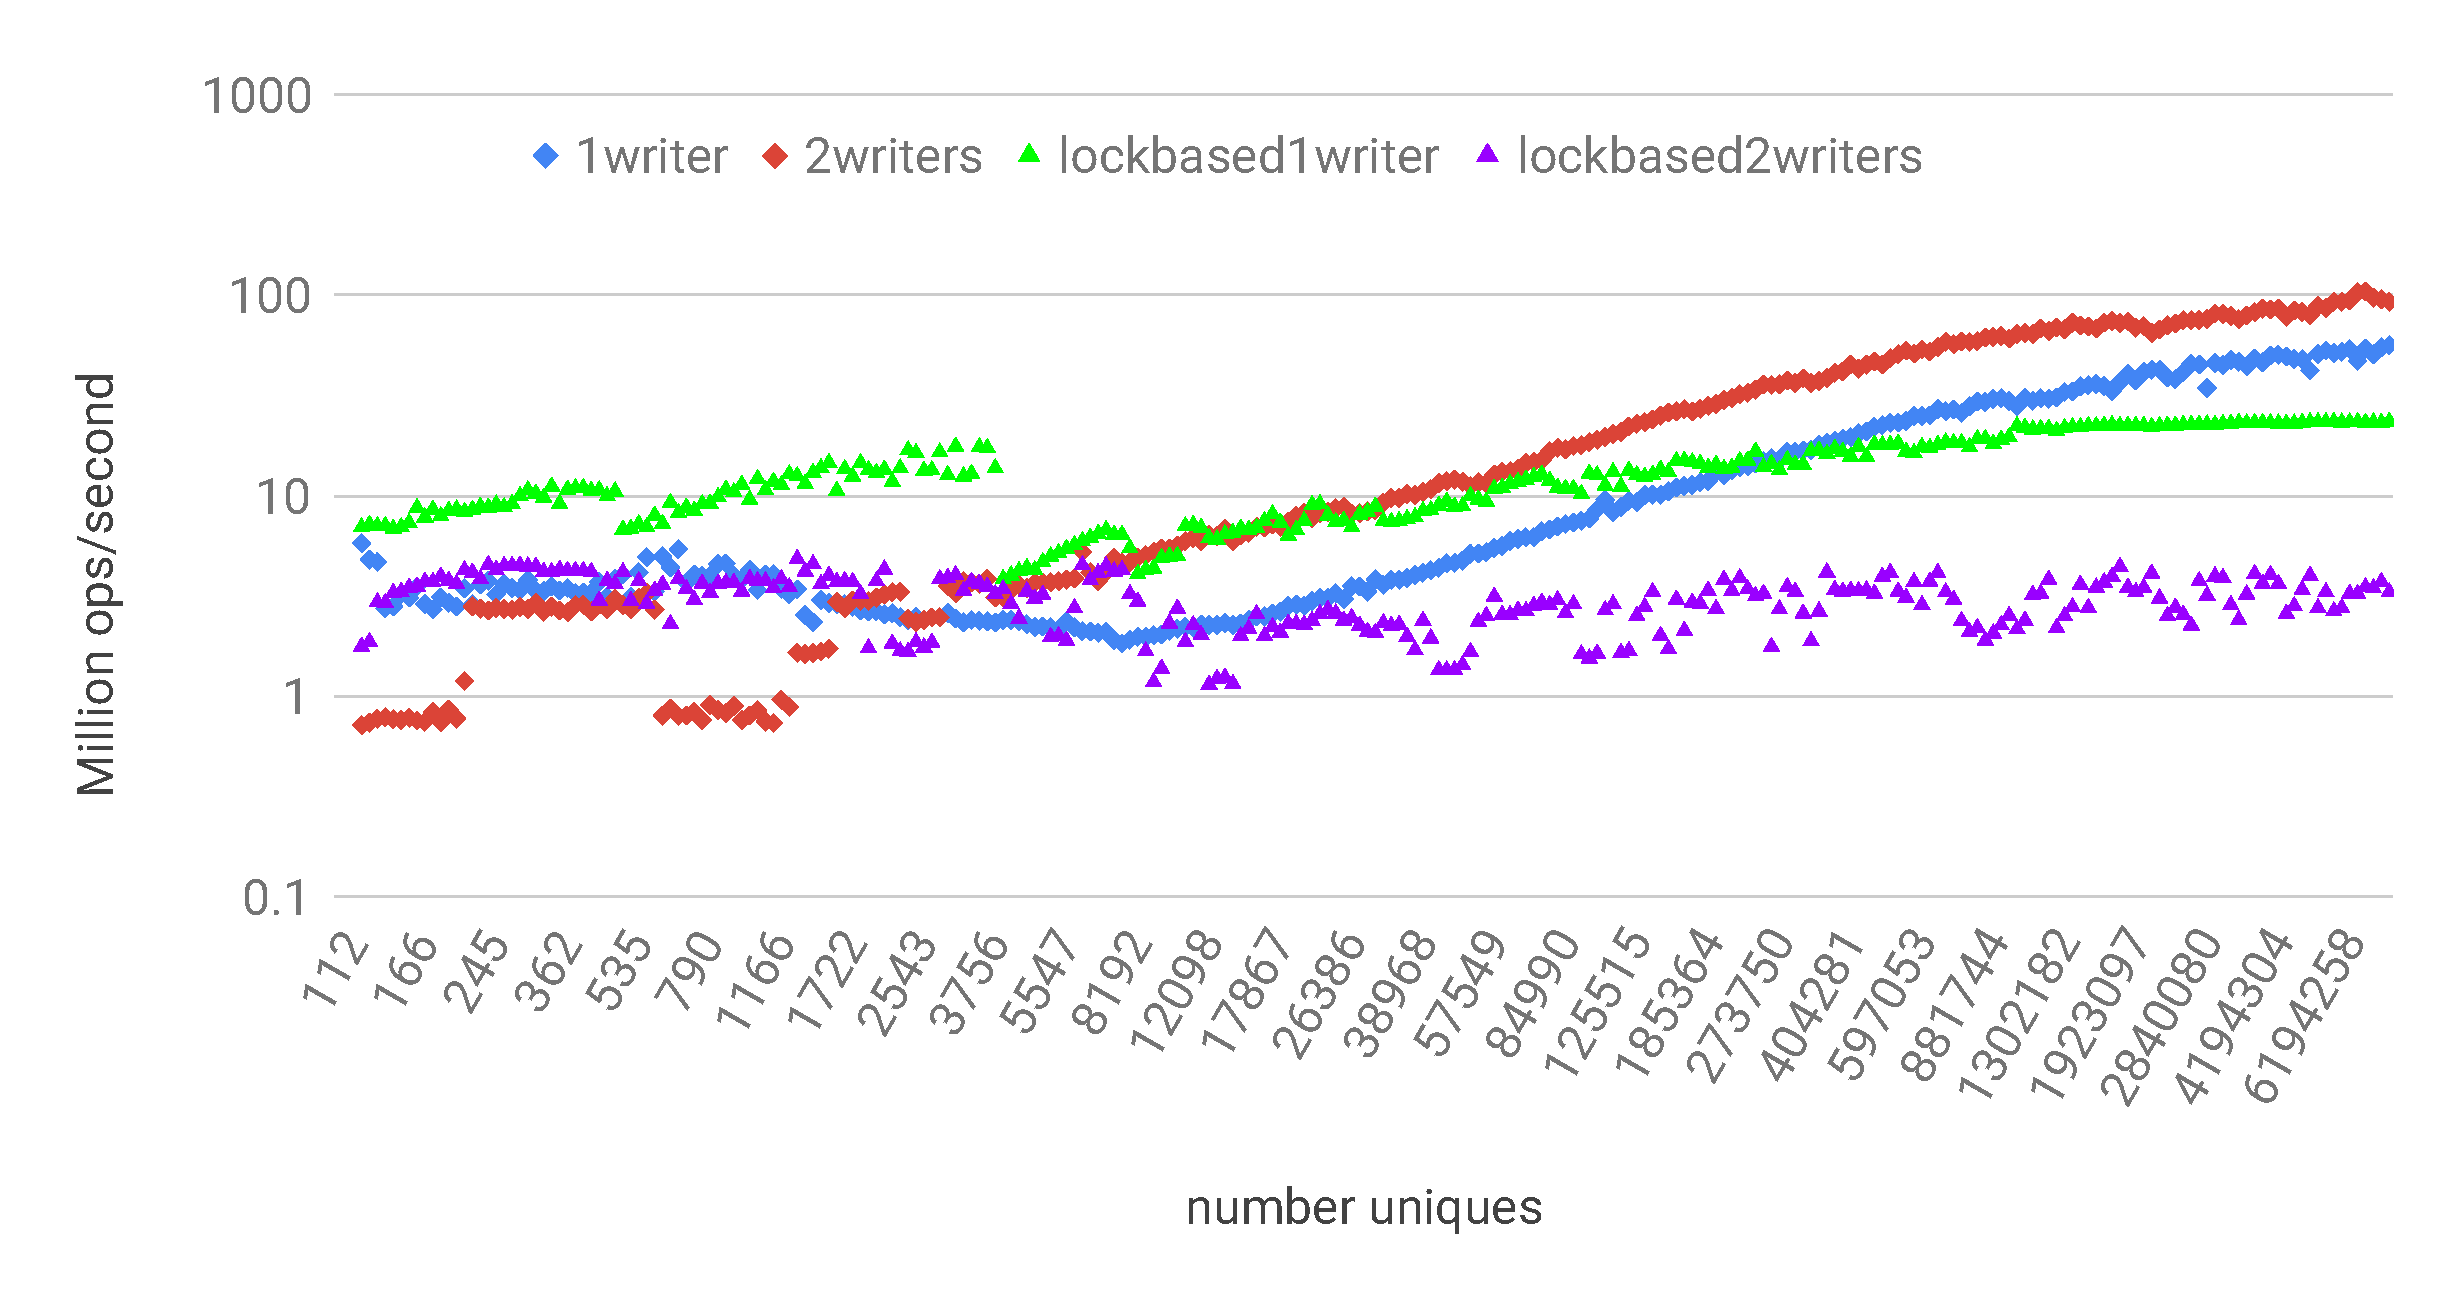
\includegraphics[width=\columnwidth]{images/theta-mixed.pdf}
	\caption{{Mixed workloads: writers with background reads, $k = 4096$, $e=0.04$.}}
	\label{fig:mixed-throughput}
\end{figure}


\subsection{Accuracy-Throughput Tradeoffs}
\label{ssec:tradeoffs}

Eager vs no-eager speedup is presented in Figure~\ref{fig:speedup}. It demonstrates the speedup of eager propagation over no-eager propagation for small streams, in addition to the accuracy benefit reported in Figure~\ref{fig:accuracy-res}. 
The improvement goes up to 84x throughput for tiny sketches, and decreases as the sketch grows. %since the improvement potential is smaller.
The slowdown in performance when the sketch size exceed $2k$ can be explained by the reduction in local buffer size (from $b=16$ to $b=5$) in order to accommodate for the required error bound.

\begin{figure}[tb]
\setlength{\abovecaptionskip}{0pt}
\setlength{\belowcaptionskip}{0pt}
\setlength\textfloatsep{0pt}
	\centering
	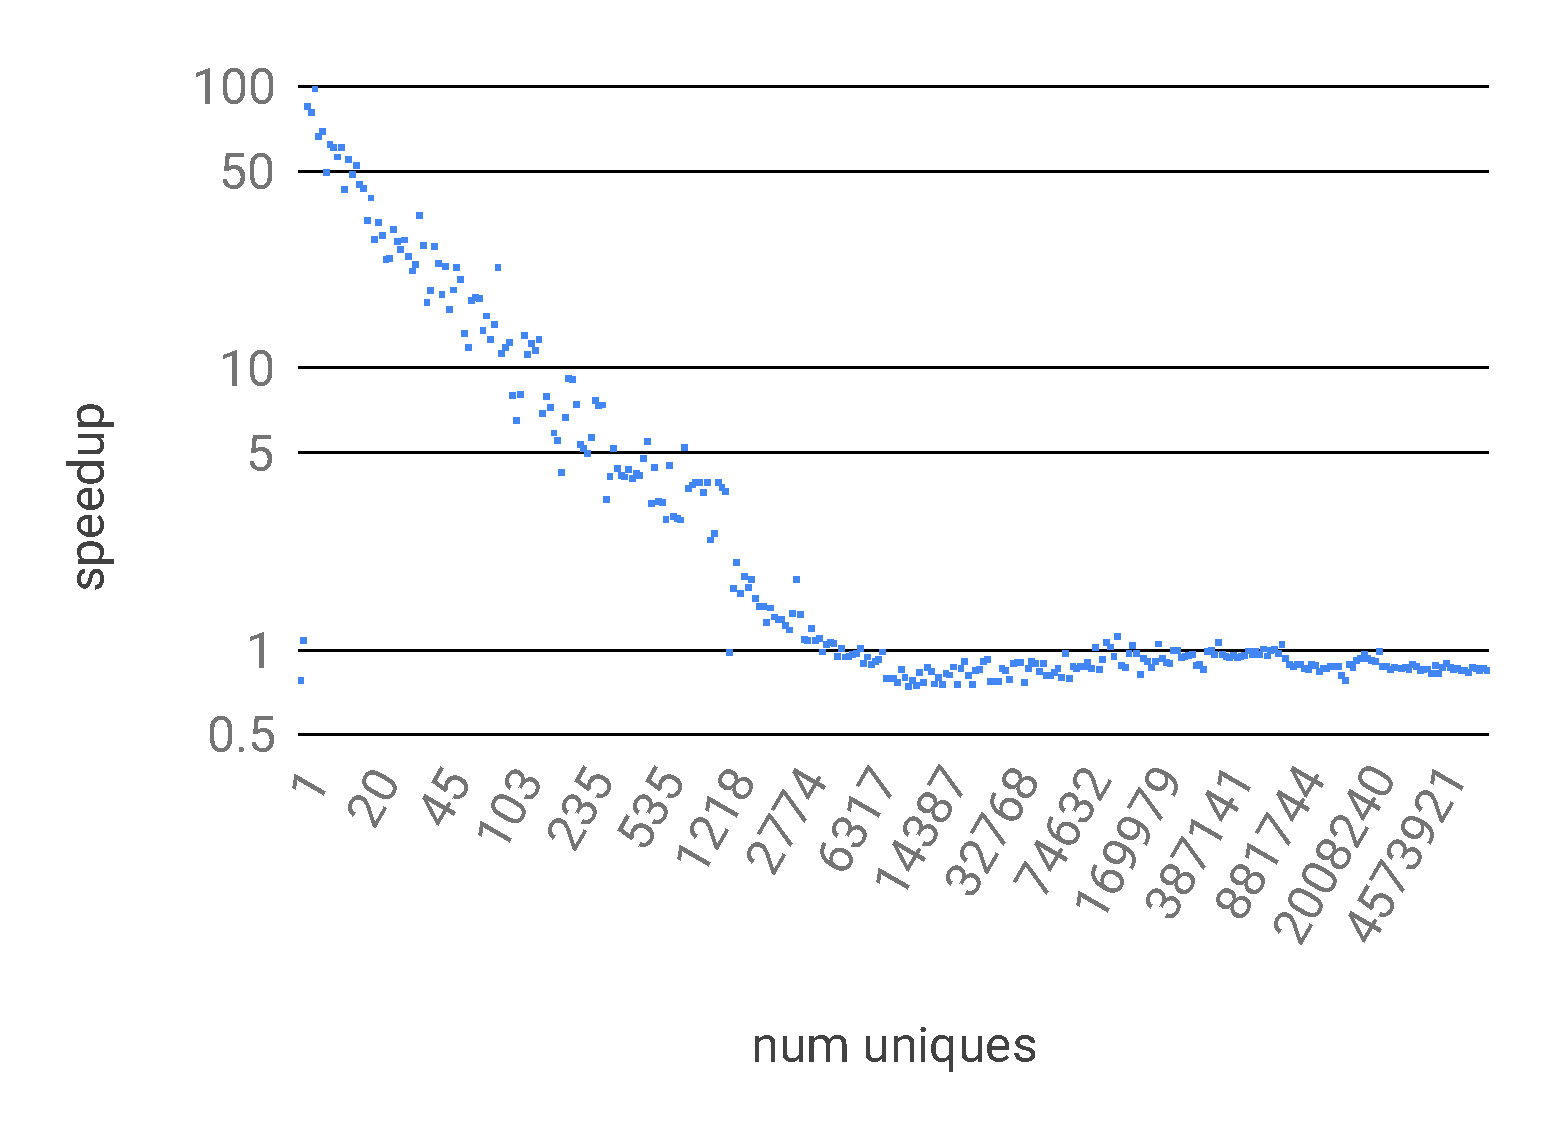
\includegraphics[width=\columnwidth]{images/eager-speedup.pdf}
	\caption{{Throughput speedup of eager ($e=0.04$) vs no-eager ($e=1.0$) propagation, $k = 4096$.}}
	\label{fig:speedup}
\end{figure}


Next we discuss the impact of $k$.
One way to increase the throughput of the concurrent $\Theta$ sketch is by increasing the size of the global sketch, namely increasing $k$. On the other hand, this change also increases the error of the estimate.
Table~\ref{tab:tradeoff} presents the tradeoffs between performance and accuracy. Specifically, it presents the crossing-point, the size of the sketch where concurrent implementation outperforms lock-based implementation (both running a single thread), the maximum values (across sketch sizes) of the median error, and 99th percentile error for a variety of $k$ values. 

\begin{table}[htb]
\center{\small{
\begin{tabular}{lrrr}
\hline 
& thpt crossing point & error $Q=0.5$ & error $Q=0.99$ \\
\hline 
$k=256$ &  15,000 &	0.16 & 0.27 \\
\hline 
$k=1024$ &  100,000 &	0.05 & 0.13 \\
\hline 
$k=4096$ & 700,000	& 0.03	& 0.05	\\ 
\hline 
\end{tabular}
}}
\caption{{Performance vs accuracy as a function of $k$}}
\label{tab:tradeoff}
\end{table}  


